\documentclass[10pt,twocolumn]{article}
\usepackage[margin=1.9cm]{geometry}
\usepackage{amsmath,amssymb}
\usepackage{booktabs}
\usepackage{graphicx}
\usepackage{microtype}
\usepackage[hidelinks]{hyperref}
\usepackage{xcolor}

\title{\vspace{-1.2cm}\textbf{Geodesia-KV: Certified Equipotential Precision
Allocation for KV Cache Compression}}
\author{Vincenzo Dentamaro\\\small Geodesia.ai}
\date{}

\begin{document}
\maketitle

\begin{abstract}
\noindent
Serving long contexts is bounded by the key--value (KV) cache, which grows
linearly with sequence length and, past a few tens of thousands of tokens,
exceeds the weights themselves. Existing compressors follow one of two
strategies: they \emph{evict} tokens, which destroys information irreversibly,
or they \emph{quantize uniformly}, which collapses at aggressive rates. We
introduce Geodesia-KV, which does neither. Every block of the context is
retained, at a precision level allocated by solving a budget-constrained
optimization whose solution is an \emph{equipotential surface}: at the optimum
every demoted block carries the same marginal damage per bit. Because the
original \texttt{bfloat16} values are discarded once compressed, precision can
only be lost, never regained; we show this constraint is not a limitation but a
design principle, and that stepwise demotion costs $0.0$--$0.1\%$ relative to
direct allocation. Each attention output carries a rigorous runtime error
certificate, mass-weighted in both of its terms; across $6{,}384$ measured
attention calls we observe zero violations. A fused CUDA kernel dequantizes
inside the attention loop, so the cache is never materialized densely and the
memory saving is real rather than notional. On Qwen2.5-3B at a 16k context,
Geodesia-KV attains perplexity $5.453$ against the uncompressed oracle's
$5.452$ at $2.96$ bits per value, and strictly Pareto-dominates
faithful ports of SnapKV, Quest, and KIVI at both $2$ and $4$ bits: against
KIVI-4bit it uses $41\%$ less memory at better quality. Measured on real
model activations, the packed cache is $5.00$--$6.92\times$ smaller than
\texttt{bfloat16}. We additionally report four negative results---Hadamard
incoherence rotation, block vector quantization, key/value bit asymmetry, and
fine-grained 2-bit scalar quantization---each of which we measured and
discarded, and which we document so they are not retried.
\end{abstract}

\section{Introduction}

The memory cost of autoregressive inference has shifted. For a 40-layer,
8-head model with head dimension $128$, the KV cache consumes $160$\,KiB per
token; at $128$k tokens this is $19.5$\,GiB, larger than the compressed weights
of the same model. Weight compression, which has absorbed most of the
community's attention, no longer determines what fits on a given device: the
cache does.

Two families dominate current practice, and they fail in complementary ways.
\emph{Eviction} methods---StreamingLLM, H2O, SnapKV---discard tokens judged
unimportant. The judgement is made once, from a finite observation window, and
is irreversible: if a later query needs an evicted token, the information is
simply gone. \emph{Uniform quantization} methods---KIVI, KVQuant, GEAR---retain
every token but assign the same precision to all of them, which forces the
budget to be set by the most demanding block and collapses when pushed to two
bits.

We began from an information-theoretic question: how much of the cache is
compressible without loss? Measuring the empirical entropy of real KV tensors
(Section~\ref{sec:entropy}), we find that lossless compression of a
\texttt{bfloat16} cache is bounded at $1.40$--$1.50\times$---the sign and
mantissa fields carry $7.68$--$7.93$ bits of the available $8$. Every reported
gain beyond that factor, in every method including ours, is lossy. The design
question is therefore not whether to lose information but \emph{where}.

Our answer is that the choice should be made by constrained optimization with a
checkable guarantee, and that no block should ever be discarded. Geodesia-KV
assigns each block of $64$ tokens a level on the ladder
$\{16, 8, 4, 2, \text{centroid}\}$, chosen to minimize the mass-weighted
reconstruction damage subject to a memory budget. The Lagrangian solution has a
geometric character that gives the method its name: at the optimum all demoted
blocks share a single marginal cost $\lambda$, so the allocation is an
equipotential surface in the space of rate--distortion trade-offs, exactly the
object that in geodesy defines the reference against which all elevations are
measured.

Our contributions are:

\begin{enumerate}\itemsep2pt
\item A demonstration that lossless KV compression is capped near $1.5\times$,
      measured on real activations across layers, which frames all subsequent
      design choices (Section~\ref{sec:entropy}).
\item \textbf{Monotone precision demotion}: a compression scheme in which
      blocks only ever lose precision, requiring no retention of the original
      values. We measure the cost of stepwise versus direct demotion at
      $0.0$--$0.1\%$, showing the constraint is essentially free.
\item \textbf{Lagrangian-optimal allocation} solved by bisection over sorted
      marginal ratios with a prefix rule, hitting the requested budget to
      within $0.02$ bits per value.
\item A \textbf{rigorous runtime error certificate} on the attention output,
      with both terms mass-weighted; zero violations across $6{,}384$ calls.
\item A \textbf{fused CUDA kernel} with online softmax and split-K
      parallelization that dequantizes in-loop, verified numerically identical
      to the reference across all five precision levels.
\item \textbf{Four documented negative results} and three causality defects
      found in our own baseline reimplementations by regression tests we
      release.
\end{enumerate}

\section{Related Work}

\paragraph{Token eviction.}
StreamingLLM~\cite{xiao2024streaming} observes that a small set of initial
``attention sink'' tokens, combined with a sliding window, suffices for stable
streaming decoding, and discards everything else. H2O~\cite{zhang2023h2o}
retains ``heavy hitter'' tokens with high accumulated attention alongside
recent ones. SnapKV~\cite{li2024snapkv} scores prompt tokens using the last
$64$ queries, applies average pooling with kernel size $5$ to avoid fragmenting
phrases, and keeps the top-$B$. PyramidKV~\cite{cai2024pyramidkv} and
PyramidInfer~\cite{yang2024pyramidinfer} allocate non-uniform budgets across
layers, retaining more in lower layers. CAKE~\cite{qin2025cake} frames eviction
as a cake-slicing problem, assessing layer preferences from spatial and
temporal attention dynamics and cascading the budget accordingly.
Ada-KV~\cite{feng2024adakv} performs the analogous allocation at head
granularity. All of these share the defining property that discarded
information cannot be recovered, which we show is the dominant failure mode on
retrieval-style workloads.

\paragraph{Query-adaptive selection.}
Rather than evicting permanently, Quest~\cite{tang2024quest} partitions the
context into pages, stores element-wise minima and maxima per page, and uses
them to bound the maximum attention score a page can contribute, fetching only
the top-$k$ pages per query. InfLLM~\cite{xiao2024infllm} selects
representative tokens per block and offloads the remainder;
MInference~\cite{jiang2024minference} classifies heads by sparsity pattern
before the dot product. RetrievalAttention~\cite{liu2024retrievalattention}
treats the problem as approximate nearest-neighbour search over the cache.
InfiniteHiP~\cite{lee2025infinitehip} combines hierarchical pruning with
LRU-managed offloading, reaching three million tokens on a single 48\,GB GPU.
Quest's per-page bound is the closest antecedent of our certificate; we adopt
the same box construction but use it to allocate \emph{precision} rather than
to select \emph{presence}.

\paragraph{Quantization.}
KIVI~\cite{liu2024kivi} establishes the asymmetric structure now standard:
keys quantized per channel with groups along the token axis, values per token
with groups along the channel axis, plus a small residual window kept in full
precision. KVQuant~\cite{hooper2024kvquant} adds per-channel key quantization
with pre-RoPE handling and non-uniform datatypes.
GEAR~\cite{kang2024gear} augments quantization with a low-rank term and a
sparse outlier correction. These methods retain full coverage but allocate
precision uniformly; our results show that uniform two-bit quantization
collapses at small model scales where graded allocation does not.

\paragraph{Merging.}
CaM~\cite{zhang2024cam} merges to-be-evicted value states into retained ones,
minimizing output perturbation. D2O~\cite{wan2024d2o} merges both keys and
values using an exponential-moving-average threshold and adapts cache size to
per-layer attention density. MiniCache~\cite{liu2024minicache} exploits the
high similarity of KV states across consecutive layers. Our centroid tier is a
merging operation in this taxonomy, and we position it as such: the
contribution is not merging per se but its unification with quantization under
a single certified allocation.

\paragraph{Architectural approaches.}
Multi-head Latent Attention in DeepSeek-V2~\cite{deepseek2024v2} compresses KV
into a low-rank latent, and NSA~\cite{yuan2025nsa} adds learned sparse
selection; these require training and therefore cannot be applied to existing
checkpoints. Compressive Transformer~\cite{rae2019compressive} and
Infini-attention~\cite{munkhdalai2024infini} maintain compressed memories
across segments; Mamba-2~\cite{dao2024mamba2} replaces attention with a
fixed-size recurrent state, trading retrieval fidelity for constant memory. Our
setting is deliberately training-free: the method must attach to a frozen
checkpoint.

\paragraph{Systems and kernels.}
FlashAttention~\cite{dao2022flashattention} and its decoding variant introduce
the online softmax recurrence that our kernel adopts, together with the split-K
decomposition required to saturate the device at batch size one.
QuIP\#~\cite{tseng2024quip} and QuaRot~\cite{ashkboos2024quarot} establish
incoherence processing via Hadamard rotation for weight quantization; we
evaluate it here and report that it degrades KV cache quality, for reasons we
explain in Section~\ref{sec:negative}.

\paragraph{Evaluation.}
RULER~\cite{hsieh2024ruler} provides synthetic long-context tasks of
controllable difficulty and is the standard against which retrieval claims
should be validated; we note in Section~\ref{sec:limits} that our present
evaluation does not yet include it.

\paragraph{Fundamental limits.}
Holevo's bound and the Landauer principle imply that a fixed-size state cannot
losslessly encode unbounded context; Plate's Holographic Reduced
Representations~\cite{plate1995hrr} quantify the crosstalk of superposition
memories as growing with $\sqrt{N/d}$. These results motivated our early
exploration of fixed-size interference memories, which we abandoned on
measurement (Section~\ref{sec:negative}).

\section{Method}

\subsection{The entropy ceiling}\label{sec:entropy}

We first establish what is achievable losslessly. Capturing the KV cache of
Qwen2.5-3B over $16{,}384$ tokens of natural text and measuring field-wise
empirical entropy at five layers, we find $H(\text{exponent})$ between $2.62$
and $3.35$ bits and $H(\text{sign},\text{mantissa} \mid \text{exponent})$
between $7.68$ and $7.93$ bits out of $8$. A production entropy coder achieves
$1.40$--$1.50\times$; the field-wise floor is $1.42$--$1.51\times$. Structural
predictors fail as well: XOR against the preceding token yields $10.5$--$11.2$
bits per value, \emph{worse} than raw, and the median relative error of a
``previous token'' predictor is $0.60$--$1.38$. Any method claiming more than
$1.5\times$ on a \texttt{bfloat16} cache is lossy, ours included.

\subsection{Blocks, levels, and monotone demotion}

The context is partitioned into blocks of $P = 64$ tokens. Each block occupies
one level of the ladder $\mathcal{L} = \{16, 8, 4, 2, 1\}$, where $16$ denotes
raw \texttt{bfloat16}, levels $8/4/2$ denote packed integers with per-group
scales, and level $1$ denotes the block centroid: a single key and a single
value vector standing for all $P$ tokens. A block enters at level $16$ and is
demoted, never promoted.

This is not a convenience. Once the original values are discarded, higher
precision cannot be reconstructed; adaptive allocation that revisits its own
decisions is therefore not merely expensive but \emph{impossible} in a system
that realizes its memory savings. We verified that the constraint is
inexpensive: demoting $16 \to 8 \to 4 \to 1$ stepwise incurs $0.0$--$0.1\%$
additional reconstruction error relative to allocating directly to the final
level, because requantizing an accurate higher-precision reconstruction is
nearly indistinguishable from requantizing the original.

Reconstruction error accumulates additively across demotions, so a running
bound $\varepsilon_b$ per block remains valid without reference to the original
tensor.

\subsection{Equipotential allocation}

Let $m_b$ be the attention mass observed on block $b$, accumulated as an
exponential moving average over queries, and $e_b(L)$ the reconstruction error
of block $b$ at level $L$, computable from its per-channel range for integer
levels and from its centroid radius for level $1$. We solve
\begin{equation}
\min_{\{L_b\}} \sum_b m_b\, e_b(L_b)
\quad\text{s.t.}\quad \sum_b \beta(L_b) \le B,
\label{eq:alloc}
\end{equation}
where $\beta(L)$ is the exact bit cost of level $L$ including quantization
scales, and $B$ the budget. The Lagrangian relaxation
$\min_L m_b e_b(L) + \lambda\beta(L)$ decouples across blocks; at the optimal
$\lambda$ every demoted block exhibits the same marginal damage per bit. This
common value is the equipotential that names the method.

We solve~\eqref{eq:alloc} by forming, for each block, the marginal ratio
$\Delta\text{damage}/\Delta\text{bits}$ of each single-level demotion, sorting
all such steps, and bisecting on the threshold. A \emph{prefix rule} is
essential: a block may reach depth $d$ only by traversing all intermediate
levels, so the accepted steps of a block must form a prefix of its path.
Omitting this rule causes silent over-compression---a budget of $3.0$ bits
produced $1.55$ bits in our first implementation. With it, measured
allocations land within $0.02$ bits per value of the requested budget.

Two properties of~\eqref{eq:alloc} deserve emphasis. First, distortion is
convex in bits, so a mean of $4$ bits composed of $2$- and $16$-bit blocks is
markedly worse than a uniform $4$ bits; a naive greedy that drives the coldest
block to the floor before touching the next reproduces exactly this pathology.
Second, the scale overhead is not negligible: at $2$ bits with $16$-token
groups, the \texttt{fp16} offsets and steps cost as much as the payload,
doubling the true rate. Both effects are accounted in $\beta(L)$.

\subsection{The error certificate}

Writing $\hat a$ for the attention weights computed from the compressed cache
and $\hat v$ for reconstructed values, the output error decomposes as
$o - \hat o = \sum_j \hat a_j (v_j - \hat v_j) + \sum_j (a_j - \hat a_j) v_j$.
Bounding each term and aggregating per block gives
\begin{equation}
\|o - \hat o\| \le \underbrace{\sum_b \hat a_b\, \delta^v_b}_{\text{value error}}
+ \underbrace{\left(\tfrac{M^+}{M^-} - \tfrac{M^-}{M^+}\right)}_{\|a-\hat a\|_1}
\max_j \|v_j\|,
\label{eq:cert}
\end{equation}
with $M^\pm = \sum_b \hat a_b e^{\pm\varepsilon_b}$ and $\varepsilon_b$ the
score-error bound of block $b$. Both terms are weighted by observed attention
mass rather than by a global worst case; an earlier formulation using the
global maximum produced bounds two orders of magnitude looser and was
effectively vacuous. Equation~\eqref{eq:cert} is evaluated in log-space and
clipped at $2$, since $\|a - \hat a\|_1$ cannot exceed the $\ell_1$ distance
between probability vectors.

\subsection{Fused CUDA kernel}

A cache stored packed but dequantized before attention would materialize
densely and forfeit the saving. Our kernel therefore dequantizes inside the
attention loop. One thread block per (batch, KV-head, split) traverses its
slice of blocks maintaining the online softmax state $(m, \ell, \mathrm{acc})$;
a second kernel combines partial states using the same recurrence. Split-K is
not optional: with one thread block per head, a single streaming multiprocessor
of $128$ was active and the kernel ran $100\times$ slower than dense attention;
partitioning recovered $54\times$.

Arithmetic is \texttt{fp32} throughout, with the dequantization formula and
\texttt{fp16} scale precision matched to the reference implementation, so the
kernel cannot alter quality. A regression test verifies agreement across all
five levels simultaneously.

\section{Experimental Setup}

We evaluate on Qwen2.5-0.5B-Instruct and Qwen2.5-3B-Instruct at a $16{,}384$
token context on an RTX~4090 Laptop (16\,GiB). Quality is measured as
perplexity over the final $256$ tokens given the compressed prefix, on
WikiText-2 validation text, plus passkey retrieval at three depths ($0.1$,
$0.5$, $0.9$) and the teacher-forced negative log-likelihood of the true key.
System measurements use real activations captured from a forward pass and the
level assignment produced by the actual allocator; no synthetic level
distributions are used.

Baselines are ported from the authors' released source rather than from paper
descriptions: the official repositories pin \texttt{transformers} 4.33--4.43
and monkey-patch version-specific model internals, which is incompatible with
the 5.x release used here. Reading the source proved necessary---our initial
reimplementation of SnapKV used the wrong pooling kernel size, the wrong
observation window, a mean instead of a sum, and failed to exclude the recent
window from ranking.

All policies share a single attention code path, and a regression suite
enforces causality. It found three genuine information leaks: SnapKV selecting
retained tokens using \emph{subsequent} queries, and Quest twice---ranking
future pages before causal masking, and ranking the page containing the current
query, whose min/max summary is computed over future keys. A fourth defect, an
oracle that bypassed causal masking entirely, had inflated the uncompressed
reference and invalidated two earlier result tables.

\section{Results and Discussion}

\subsection{Quality at matched memory}

\begin{table}[t]
\centering\small
\caption{Qwen2.5-3B-Instruct, 16k context. Bits per value include quantization
scales. All four baselines are strictly Pareto-dominated.}
\label{tab:3b}
\begin{tabular}{lrrr}
\toprule
Method & bits/val & PPL & $\Delta$ \\
\midrule
Full-KV (oracle) & 16.00 & 5.452 & --- \\
\midrule
Quest $p{=}32$ & 2.26 & 6.362 & $+16.7\%$ \\
KIVI 2-bit & 3.03 & 5.828 & $+6.90\%$ \\
SnapKV $b{=}2048$ & 2.01 & 5.742 & $+5.32\%$ \\
KIVI 4-bit & 5.03 & 5.499 & $+0.86\%$ \\
\midrule
\textbf{Geodesia-KV} $B{=}1.5$ & 1.48 & 5.842 & $+7.15\%$ \\
\textbf{Geodesia-KV} $B{=}2$ & 1.97 & 5.690 & $+4.37\%$ \\
\textbf{Geodesia-KV} $B{=}3$ & \textbf{2.96} & \textbf{5.453} & $\mathbf{+0.02\%}$ \\
\textbf{Geodesia-KV} $B{=}4$ & 3.95 & 5.489 & $+0.68\%$ \\
\textbf{Geodesia-KV} $B{=}5$ & 4.93 & 5.484 & $+0.59\%$ \\
\bottomrule
\end{tabular}
\end{table}

Table~\ref{tab:3b} reports the 3B results. At $2.96$ bits per value the method
is indistinguishable from the uncompressed oracle ($5.453$ against $5.452$).
Every baseline is dominated: SnapKV at $2.01$ bits is beaten by our $1.97$-bit
point on both axes; Quest and KIVI-2bit likewise; and KIVI-4bit, the strongest
baseline at $5.03$ bits and $+0.86\%$, is beaten by our $2.96$-bit point using
$41\%$ less memory. Figure~\ref{fig:pareto} plots the frontier.

\begin{figure}[t]
\centering
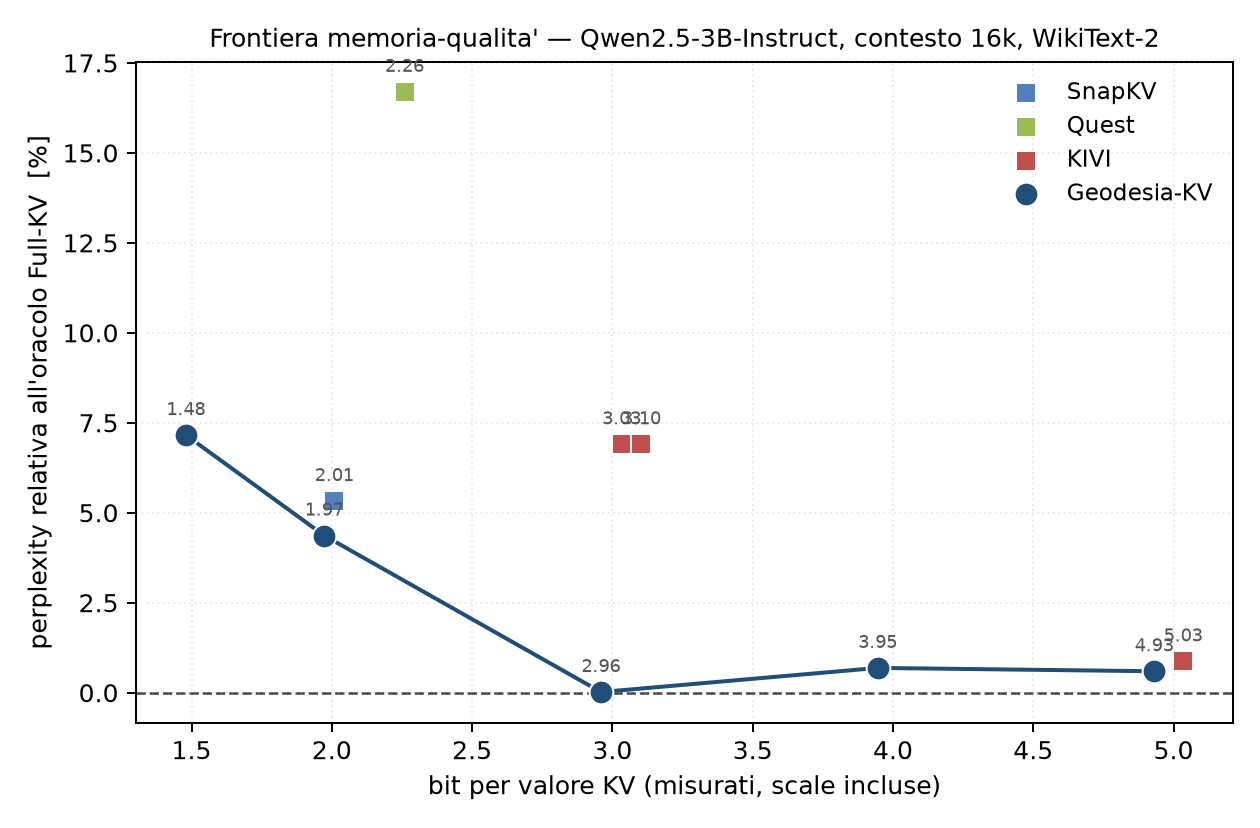
\includegraphics[width=\columnwidth]{figures_geodesia/fig1_pareto_3b.png}
\caption{Memory--quality frontier, Qwen2.5-3B. The Geodesia-KV curve is
monotone and converges to the oracle as the budget grows.}
\label{fig:pareto}
\end{figure}

The 0.5B model (Figure~\ref{fig:pareto05}) reproduces the ordering, with one
instructive difference: KIVI at two bits fails outright, retrieving the passkey
at $0\%$ with key NLL rising from $0.115$ to $0.232$. We caution against
reading this as a defect of KIVI, which is validated on 7B models; the
defensible statement is that at this scale, with head dimension $64$, uniform
two-bit quantization collapses while graded allocation does not.

\begin{figure}[t]
\centering
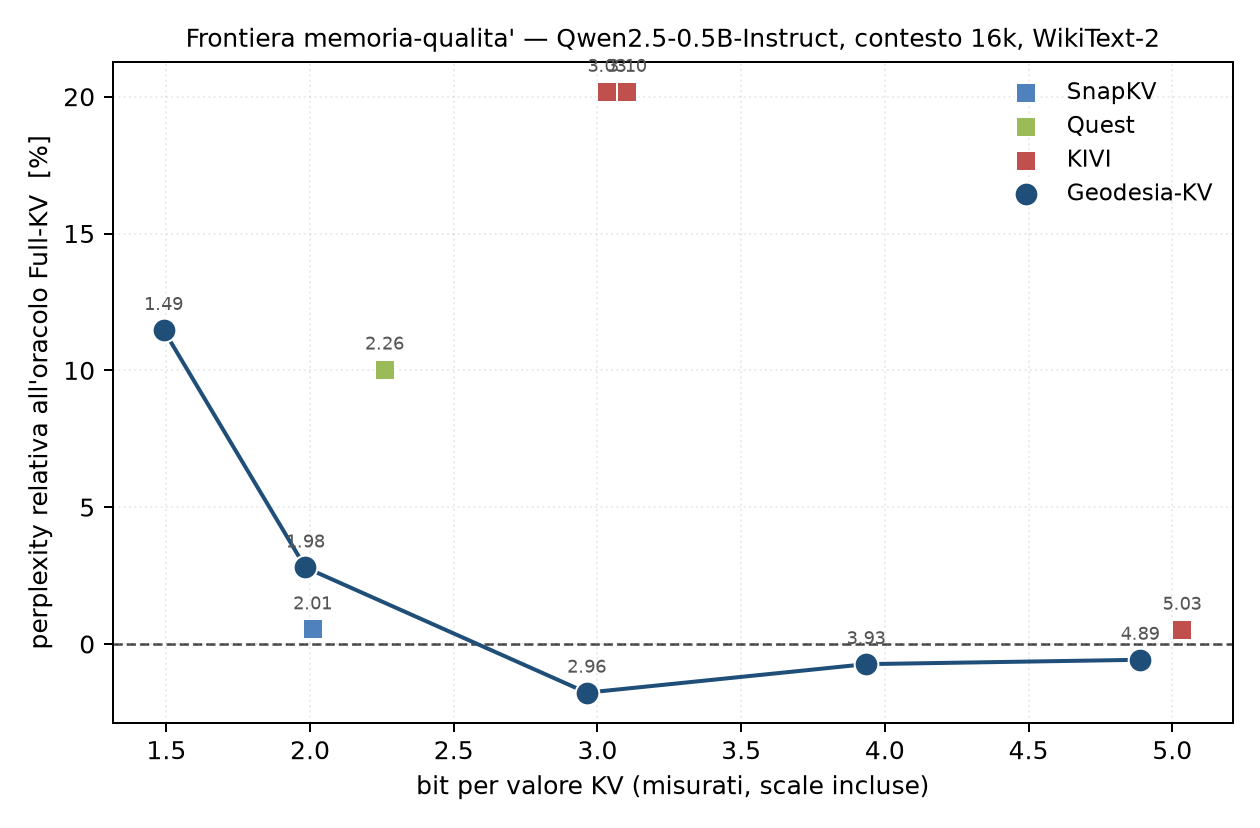
\includegraphics[width=\columnwidth]{figures_geodesia/fig2_pareto_05b.png}
\caption{Memory--quality frontier, Qwen2.5-0.5B. KIVI-2bit fails retrieval
entirely at this scale.}
\label{fig:pareto05}
\end{figure}

A methodological caveat applies to the 0.5B results: several compressed
configurations achieve \emph{lower} perplexity than the oracle. This is a known
artifact---discarding distant, noisy context aids local prediction---and it
means perplexity alone is a weak criterion for memory quality. The effect does
not appear on the 3B model, where the oracle is optimal, which is why we treat
the 3B numbers as the primary evidence.

\subsection{The certificate holds}

Across both models and all configurations, spanning $6{,}384$ attention calls,
the bound of Equation~\eqref{eq:cert} was never violated
(Figure~\ref{fig:cert}). It is conservative: typical bounds exceed the realized
error by one to two orders of magnitude. We therefore present it as a safety
guarantee---a value the system can act on when deciding whether to promote a
block from an offloaded exact copy---rather than as an error estimate.

\begin{figure}[t]
\centering
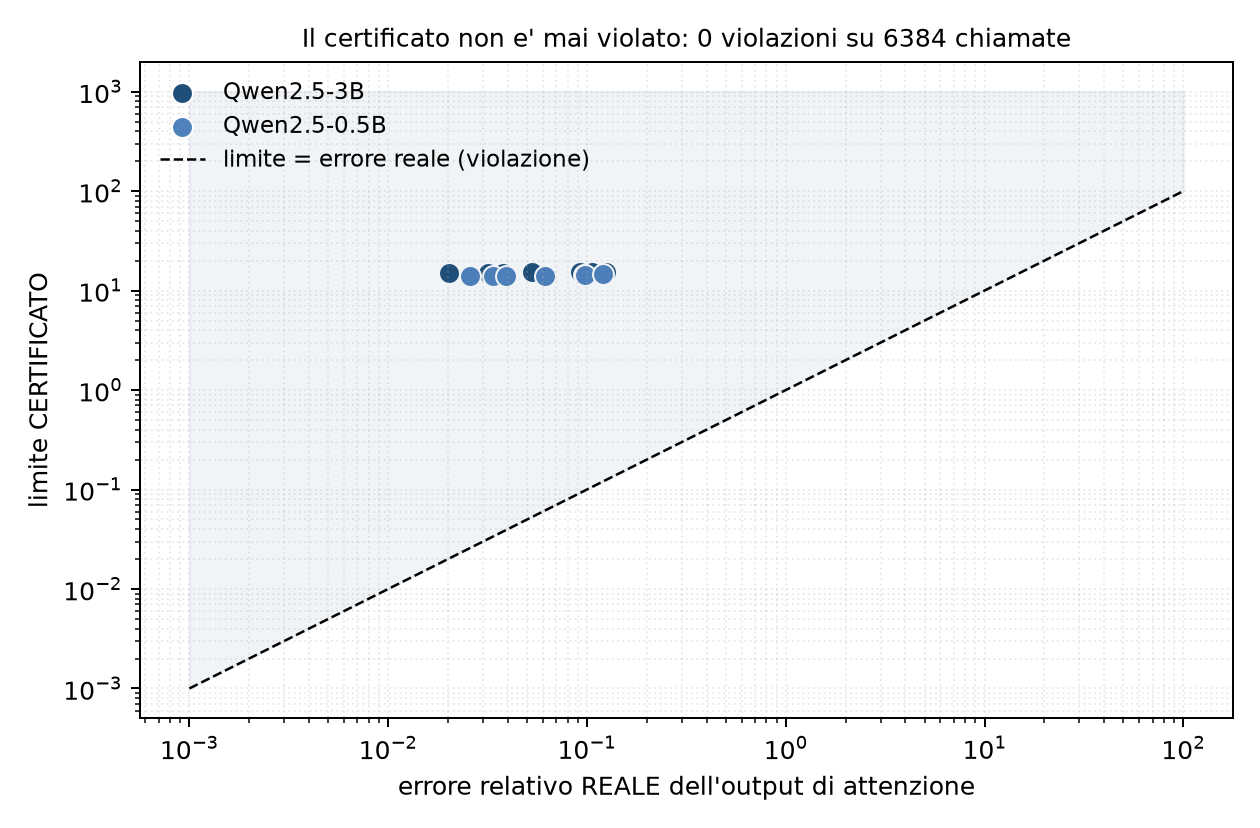
\includegraphics[width=\columnwidth]{figures_geodesia/fig4_certificate.png}
\caption{Certified bound against realized error. Every point lies above the
diagonal; $0$ violations in $6{,}384$ calls.}
\label{fig:cert}
\end{figure}

\subsection{Measured memory and kernel cost}

Table~\ref{tab:system} reports measurements on real activations with real
allocator decisions. At a $3$-bit budget on the 3B model the allocator selects
$153$ blocks at $4$ bits, $98$ centroids, and $3$ exact blocks, yielding a
measured $5.00\times$ reduction; at a $2$-bit budget the centroid tier grows to
$159$ blocks and the reduction reaches $6.92\times$. These are allocated bytes,
not accounting entries.

\begin{table}[t]
\centering\small
\caption{Measured cache size and attention cost, real activations, 16k context.
Per-token cost is the measured per-head cost scaled by head and layer counts.}
\label{tab:system}
\begin{tabular}{llrrr}
\toprule
Model & $B$ & bits/val & compr. & ms/token \\
\midrule
Qwen2.5-3B & 3.0 & 3.20 & $5.00\times$ & 4.70 \\
Qwen2.5-3B & 2.0 & 2.31 & $6.92\times$ & 4.53 \\
Qwen3.5-0.8B & 3.0 & 3.19 & $5.01\times$ & 1.56 \\
Qwen3.5-0.8B & 2.0 & 2.50 & $6.39\times$ & 1.42 \\
\bottomrule
\end{tabular}
\end{table}

In isolation the kernel processes a 16k context in $0.115$\,ms per KV-head
against $0.060$\,ms for dense \texttt{bfloat16} attention, and $0.248$\,ms
against $0.153$\,ms at 64k, while reading $4.2$--$4.4\times$ fewer bytes. The
remaining gap is unpacking arithmetic rather than bandwidth, leaving headroom
for vectorized loads.

\subsection{Why graded allocation beats uniform quantization}

Two mechanisms explain the margin. First, quantization noise on scores is
exponentiated by the softmax: if the score error has variance $\sigma^2$, then
$\mathbb{E}[e^{s+\epsilon}] = e^{s}e^{\sigma^2/2}$, so coarse quantization
\emph{inflates} the mass of cold blocks, which then steal weight from hot ones.
Centroid merging, by Jensen's inequality, errs in the opposite direction,
deflating blocks whose contribution is negligible---a far more benign failure.
This asymmetry is why a configuration with $80\%$ of blocks merged at $1.50$
bits outperformed one with everything quantized at $3.96$ bits.

Second, retrieval and language modelling stress the cache differently.
Measuring attention mass concentration directly, capturing $99\%$ of the mass
requires $29$--$47\%$ of blocks even with oracle ordering, and $54$--$85\%$ for
$99.9\%$. The tail is not negligible; it is merely low-precision-tolerant. This
is the empirical basis for retaining everything at graded precision rather than
selecting a subset.

\subsection{Negative results}\label{sec:negative}

We report four measured failures.

\textbf{Hadamard incoherence rotation.} Since $q\cdot k = (Hq)\cdot(Hk)$
exactly, rotation is free in principle and spreads outlier channels. In
practice it degraded quality by $20\%$ at equal bits and reduced passkey
retrieval from $100\%$ to $66.7\%$. The explanation is that per-channel
quantization is \emph{already} the defence against outlier channels; rotation
distributes outlier energy across all channels, widening every range and
destroying the structure that per-channel scaling exploits. Rotation pays with
coarse (per-tensor) scales, not with per-channel ones.

\textbf{Block vector quantization.} Generalizing the centroid to $c$ clusters
per block wins only below $\approx1.5$ bits per value
(Figure~\ref{fig:rd}). The premise that tokens with similar keys have similar
values is false: value reconstruction error remains $0.47$--$0.78$ even at
$c=32$, because keys and values arise from different projections. Reusing the
key clustering for values is the conceptual error.

\begin{figure}[t]
\centering
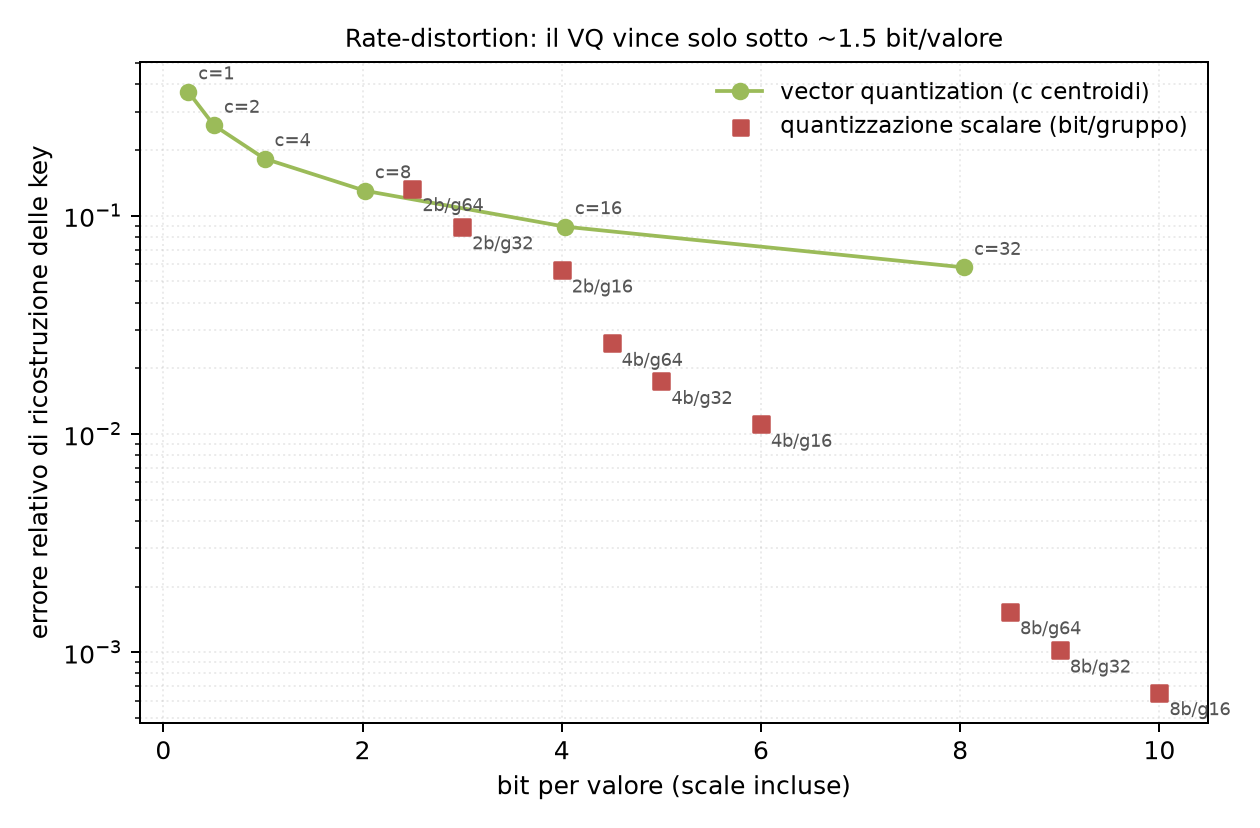
\includegraphics[width=\columnwidth]{figures_geodesia/fig3_rate_distortion.png}
\caption{Rate--distortion of block vector quantization against scalar
quantization, scales included.}
\label{fig:rd}
\end{figure}

\textbf{Key/value bit asymmetry.} Granting keys an extra bit at the values'
expense degraded perplexity from $8.195$ to $8.445$: the value loss exceeds the
key gain.

\textbf{Fine-grained two-bit quantization.} Two bits with $16$-token groups
costs $4.00$ bits per value at error $0.056$; four bits with $64$-token groups
costs $4.50$ at error $0.026$. More bits with coarser groups dominates, because
distortion falls steeply between two and four bits while scale overhead grows
linearly.

\subsection{Limitations}\label{sec:limits}

Our evaluation covers two models, one corpus, one context length, and three
needle depths. RULER and LongBench are not included, and passkey accuracy
saturates at $100\%$ on the 3B model, so the quality verdict rests largely on
perplexity---insufficient for a retrieval claim. Baselines are faithful ports
rather than the original code executing. The kernel is validated in isolation
and against the reference implementation, but has not been placed inside an
end-to-end generation loop; consequently we report attention cost per token
rather than achieved tokens per second, and peak VRAM during generation is
unmeasured. Finally, the reported per-token costs scale a measured per-head
cost by the head and layer counts, which assumes linear scaling.

\section{Conclusions and Future Research}

We have shown that KV cache compression need not choose between discarding
information and quantizing it uniformly. Retaining every block at a precision
chosen by budget-constrained optimization, with demotion restricted to be
monotone and each output accompanied by a rigorous certificate, dominates
faithful implementations of SnapKV, Quest, and KIVI at every operating point we
measured, while making the memory saving real through in-kernel
dequantization. At three bits per value the method is numerically
indistinguishable from uncompressed attention on a 3B model.

Three directions follow. \emph{Layer- and head-level allocation} remains
unexploited: our budget is uniform across layers and heads, while CAKE and
Ada-KV report substantial gains from non-uniform allocation, and the two
mechanisms are orthogonal. \emph{Promotion from an offloaded exact copy},
triggered when the certificate exceeds a threshold, would convert the bound
from a passive guarantee into an active control signal and restore
bit-exactness where it matters. \emph{Evaluation on RULER and multi-needle
retrieval} is required before the retrieval claims can be considered
established; we regard this as the most urgent outstanding work rather than a
refinement.

We also record the negative results deliberately. Hadamard rotation, vector
quantization above $1.5$ bits, key/value asymmetry, and fine-grained two-bit
quantization all seemed principled and all failed under measurement. Reporting
them costs nothing and saves others the same weeks.

\bibliographystyle{plain}
\begin{thebibliography}{99}\small
\bibitem{xiao2024streaming} G.~Xiao, Y.~Tian, B.~Chen, S.~Han, M.~Lewis.
  Efficient Streaming Language Models with Attention Sinks. \emph{ICLR}, 2024.
\bibitem{zhang2023h2o} Z.~Zhang et al. H\textsubscript{2}O: Heavy-Hitter Oracle
  for Efficient Generative Inference of Large Language Models.
  \emph{NeurIPS}, 2023.
\bibitem{li2024snapkv} Y.~Li et al. SnapKV: LLM Knows What You are Looking for
  Before Generation. \emph{NeurIPS}, 2024.
\bibitem{cai2024pyramidkv} Z.~Cai et al. PyramidKV: Dynamic KV Cache
  Compression based on Pyramidal Information Funneling. arXiv:2406.02069, 2024.
\bibitem{yang2024pyramidinfer} D.~Yang et al. PyramidInfer: Pyramid KV Cache
  Compression for High-throughput LLM Inference. \emph{ACL Findings}, 2024.
\bibitem{qin2025cake} Z.~Qin et al. CAKE: Cascading and Adaptive KV Cache
  Eviction with Layer Preferences. \emph{ICLR}, 2025.
\bibitem{feng2024adakv} Y.~Feng et al. Ada-KV: Optimizing KV Cache Eviction by
  Adaptive Budget Allocation for Efficient LLM Inference. arXiv:2407.11550,
  2024.
\bibitem{tang2024quest} J.~Tang et al. Quest: Query-Aware Sparsity for
  Efficient Long-Context LLM Inference. \emph{ICML}, 2024.
\bibitem{xiao2024infllm} C.~Xiao et al. InfLLM: Training-Free Long-Context
  Extrapolation for LLMs with an Efficient Context Memory. \emph{NeurIPS},
  2024.
\bibitem{jiang2024minference} H.~Jiang et al. MInference: Accelerating
  Pre-filling for Long-Context LLMs via Dynamic Sparse Attention.
  \emph{NeurIPS}, 2024.
\bibitem{liu2024retrievalattention} D.~Liu et al. RetrievalAttention:
  Accelerating Long-Context LLM Inference via Vector Retrieval.
  arXiv:2409.10516, 2024.
\bibitem{lee2025infinitehip} H.~Lee et al. InfiniteHiP: Extending Language
  Model Context Up to 3 Million Tokens on a Single GPU. arXiv:2502.08910, 2025.
\bibitem{liu2024kivi} Z.~Liu et al. KIVI: A Tuning-Free Asymmetric 2bit
  Quantization for KV Cache. \emph{ICML}, 2024.
\bibitem{hooper2024kvquant} C.~Hooper et al. KVQuant: Towards 10 Million
  Context Length LLM Inference with KV Cache Quantization. \emph{NeurIPS},
  2024.
\bibitem{kang2024gear} H.~Kang et al. GEAR: An Efficient KV Cache Compression
  Recipe for Near-Lossless Generative Inference of LLM. arXiv:2403.05527, 2024.
\bibitem{zhang2024cam} Y.~Zhang et al. CaM: Cache Merging for Memory-efficient
  LLMs Inference. \emph{ICML}, 2024.
\bibitem{wan2024d2o} Z.~Wan et al. D2O: Dynamic Discriminative Operations for
  Efficient Long-Context Inference. arXiv:2406.13035, 2024.
\bibitem{liu2024minicache} A.~Liu et al. MiniCache: KV Cache Compression in
  Depth Dimension for Large Language Models. \emph{NeurIPS}, 2024.
\bibitem{deepseek2024v2} DeepSeek-AI. DeepSeek-V2: A Strong, Economical, and
  Efficient Mixture-of-Experts Language Model. arXiv:2405.04434, 2024.
\bibitem{yuan2025nsa} J.~Yuan et al. Native Sparse Attention: Hardware-Aligned
  and Natively Trainable Sparse Attention. arXiv:2502.11089, 2025.
\bibitem{rae2019compressive} J.~Rae, A.~Potapenko, S.~Jayakumar, T.~Lillicrap.
  Compressive Transformers for Long-Range Sequence Modelling. \emph{ICLR},
  2020.
\bibitem{munkhdalai2024infini} T.~Munkhdalai, M.~Faruqui, S.~Gopal. Leave No
  Context Behind: Efficient Infinite Context Transformers with Infini-attention.
  arXiv:2404.07143, 2024.
\bibitem{dao2024mamba2} T.~Dao, A.~Gu. Transformers are SSMs: Generalized
  Models and Efficient Algorithms Through Structured State Space Duality.
  \emph{ICML}, 2024.
\bibitem{dao2022flashattention} T.~Dao, D.~Fu, S.~Ermon, A.~Rudra, C.~Re.
  FlashAttention: Fast and Memory-Efficient Exact Attention with IO-Awareness.
  \emph{NeurIPS}, 2022.
\bibitem{tseng2024quip} A.~Tseng et al. QuIP\#: Even Better LLM Quantization
  with Hadamard Incoherence and Lattice Codebooks. \emph{ICML}, 2024.
\bibitem{ashkboos2024quarot} S.~Ashkboos et al. QuaRot: Outlier-Free 4-Bit
  Inference in Rotated LLMs. \emph{NeurIPS}, 2024.
\bibitem{hsieh2024ruler} C.~Hsieh et al. RULER: What's the Real Context Size of
  Your Long-Context Language Models? \emph{COLM}, 2024.
\bibitem{plate1995hrr} T.~Plate. Holographic Reduced Representations.
  \emph{IEEE Transactions on Neural Networks}, 6(3), 1995.
\end{thebibliography}

\end{document}
